\documentclass[a2paper, 12pt]{article}
\usepackage[font={huge, bf}]{caption}
\usepackage{fontspec}
\setmainfont{Arial}
\usepackage{subcaption}
\usepackage{graphicx}
\usepackage{tikz}
\usepackage{tikzsymbols}
\usetikzlibrary{calc,patterns,shapes.geometric}
\usepackage{float}
\usepackage{pdflscape}
\usepackage{geometry}
\geometry{landscape, margin=2cm}
\captionsetup[subfigure]{justification=justified,singlelinecheck=false}
\pagestyle{empty}

\def\centerarc[#1](#2)(#3:#4:#5){\draw[#1] ($(#2)+({#5*cos(#3)},{#5*sin(#3)})$) arc (#3:#4:#5);}

\begin{document}
	\vspace*{\fill}
	\begin{figure}[!htbp]
		\centering
		\begin{subfigure}[b]{0.48\textwidth}
			\caption{Figure 1}
			\centering
			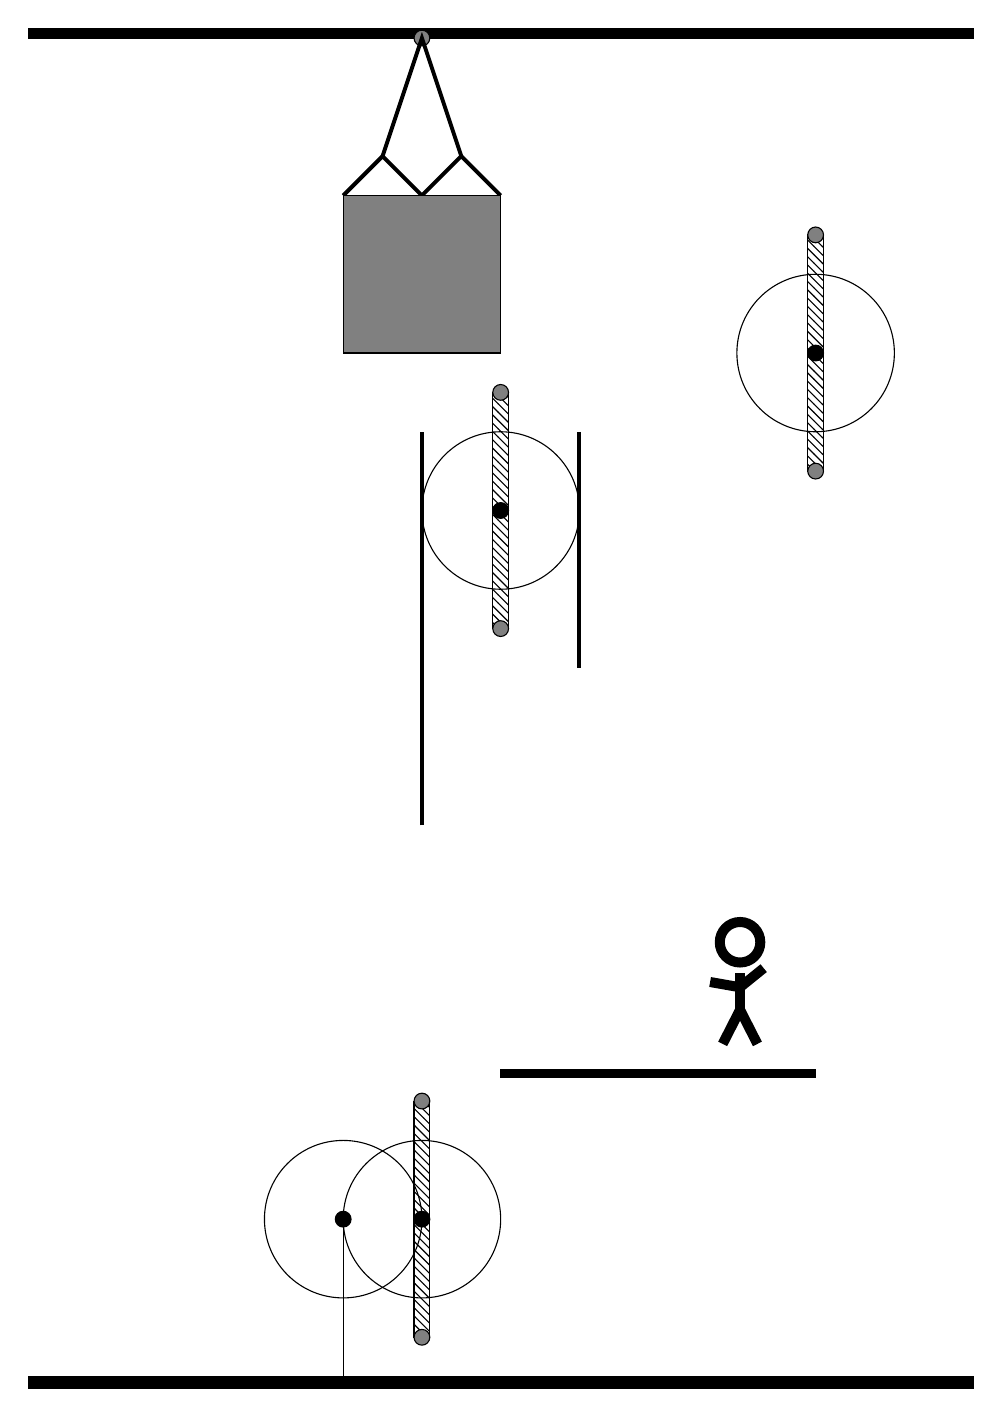
\begin{tikzpicture}
				\draw[fill=black] (-5, 14) rectangle (7, 14.125);
				
				\draw (-1,-1) circle (1);
				\draw[fill=black] (-1,-1) circle (0.1);
				\draw (-1,-3.15) -- (-1,-1);
				
				\draw (0,-1) circle (1);
				\draw[fill=black] (0,-1) circle (0.1);
				\draw[pattern=north west lines, pattern color=black] (-0.1,0.5) rectangle (0.1,-2.5);
				\draw[fill=black!50] (0,0.5) circle (0.1);
				\draw[fill=black!50] (0,-2.5) circle (0.1);
				
				\draw (5,10) circle (1);
				\draw[fill=black] (5,10) circle (0.1);
				\draw[pattern=north west lines, pattern color=black] (4.9,11.5) rectangle (5.1,8.5);
				\draw[fill=black!50] (5,11.5) circle (0.1);
				\draw[fill=black!50] (5,8.5) circle (0.1);
				
				\draw (1,8) circle (1);
				\draw[fill=black] (1,8) circle (0.1);
				\draw[pattern=north west lines, pattern color=black] (0.9,9.5) rectangle (1.1,6.5);
				\draw[fill=black!50] (1,9.5) circle (0.1);
				\draw[fill=black!50] (1,6.5) circle (0.1);
				
				\draw[fill=black!50] (0,14) circle (0.1);
				\draw[line width=0.5mm](-0.5,12.5) -- (0,14) --  (0.5,12.5);
				\draw[line width=0.5mm](-1,12) --  (-0.5,12.5) -- (0,12) -- (0.5,12.5) -- (1,12);
				\draw[fill=black!50] (-1, 12) rectangle (1, 10);
				
				\draw[line width = 0.5mm] (0,4) -- (0,9);
				\centerarc[line width = 0.5mm](1,9)(0:180:1);
				\draw[line width = 0.5mm] (2,9) -- (2,6);
				\centerarc[line width = 0.5mm](3,6)(270:180:1);
				
				\node at (4, 2) {\scriptsize \Strichmaxerl[10][-141][170]};
				\draw[fill=black] (1, 0.8999999999999999) rectangle (5, 0.8);
				
				\draw[fill=black] (-5, -3) rectangle (7, -3.15);
			\end{tikzpicture}
		\end{subfigure}
		\hfill
		\begin{subfigure}[b]{0.48\textwidth}
			\caption{Figure 2}
			\centering
			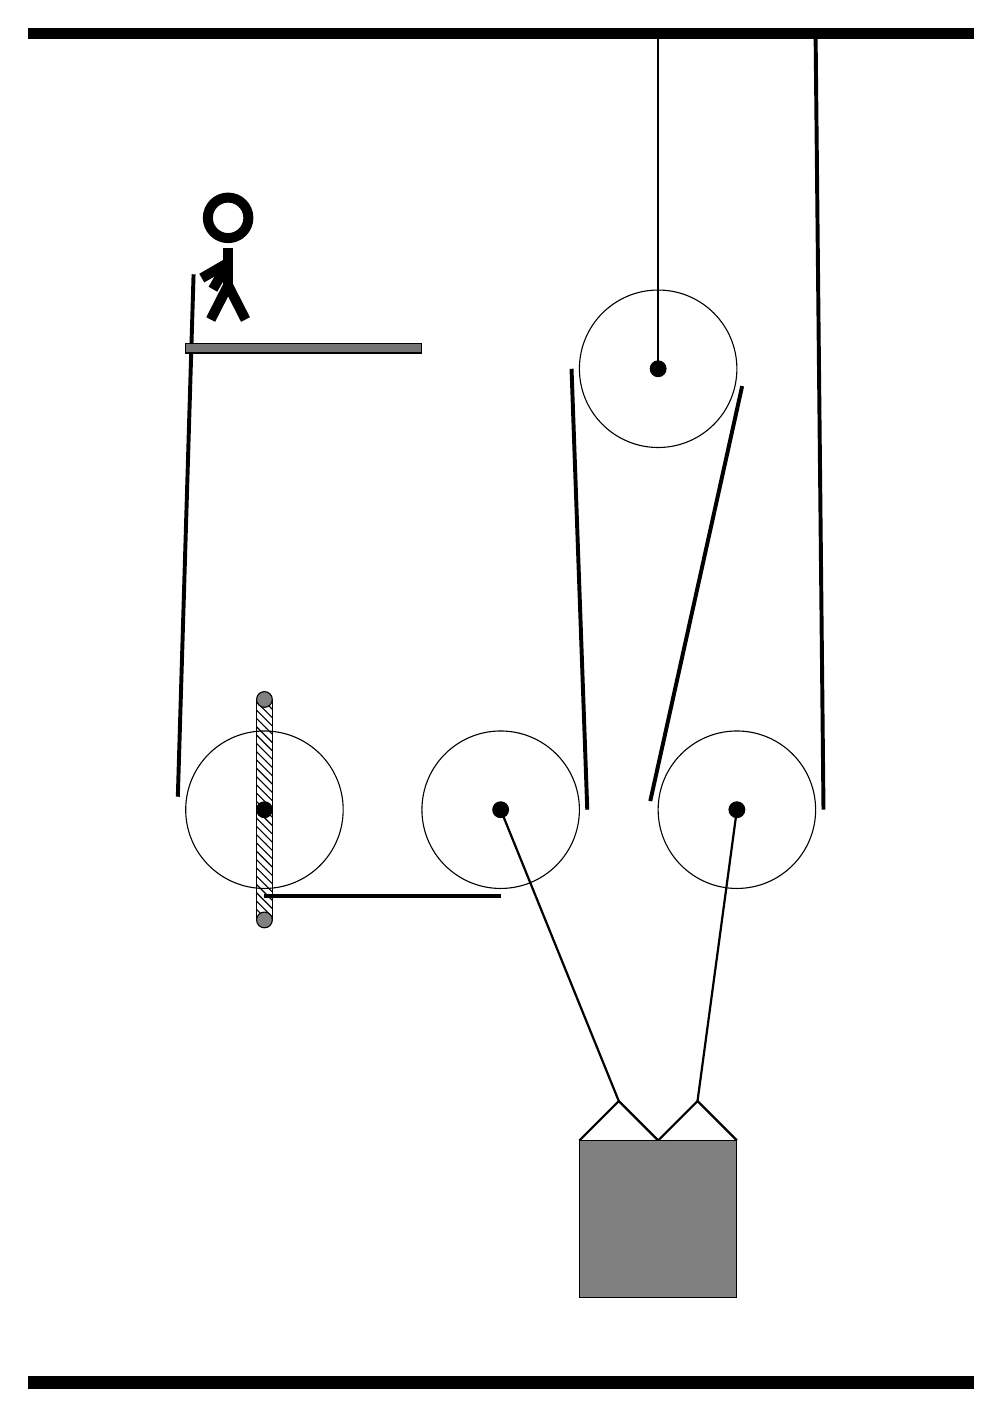
\begin{tikzpicture}
				\draw[fill=black] (-5, 14) rectangle (7, 14.125);
				
				\draw (1, 4.2) circle (1);
				\draw[fill=black] (1, 4.2) circle (0.1);
				
				\draw (3, 9.8) circle (1);
				\draw[fill=black] (3, 9.8) circle (0.1);
				\draw[thick] (3, 9.8) -- (3, 14);
				
				\draw (4, 4.2) circle (1);
				\draw[fill=black] (4, 4.2) circle (0.1);
				
				\draw[thick] (4, 4.2) -- (3.5, 0.5);
				\draw[thick] (1, 4.2) -- (2.5, 0.5);
				\draw[thick]  (2, 0) -- (2.5, 0.5) -- (3, 0);
				\draw[thick]  (3, 0) -- (3.5, 0.5) -- (4, 0);
				\draw[fill=black!50] (2, 0) rectangle (4, -2);
				
				\draw (-2, 4.2) circle (1);
				\draw[fill=black] (-2, 4.2) circle (0.1);
				\draw[pattern=north west lines, pattern color=black] (-2.1, 5.6) rectangle (-1.9, 2.8);
				\draw[fill=black!50] (-2, 5.6) circle (0.1);
				\draw[fill=black!50] (-2, 2.8) circle (0.1);
				
				\draw[line width=0.5mm] (-2.9, 11) -- (-3.1, 4.365);
				\centerarc[line width=0.5mm](-2, 4.2)(160:270:1.1);
				\draw[line width=0.5mm](-2, 3.1) -- (1, 3.1);
				\centerarc[line width=0.5mm](1, 4.2)(270:360:1.1);
				\draw[line width=0.5mm] (2.1, 4.2) -- (1.9, 9.8);
				\centerarc[line width=0.5mm](3, 9.8)(-20:180:1.1);
				\draw[line width=0.5mm](4.067, 9.58) -- (2.9, 4.31);
				\centerarc[line width=0.5mm](4, 4.2)(160:360:1.1);
				\draw[line width=0.5mm](5.1, 4.2) -- (5.0, 14);
				
				\node at (-2.5, 11.2) {\scriptsize \Strichmaxerl[10][30][-120]};
				\draw[fill=black!55] (-3, 10) rectangle (0, 10.125);
				
				\draw[fill=black] (-5, -3) rectangle (7, -3.15);
			\end{tikzpicture}
		\end{subfigure}
	\end{figure}
		\vspace*{\fill}
\end{document}